\chapter{绪论}
\label{cha:intro}

\section{研究背景及意义}

自万维网创始人Time Berner-Lee于1998年提出语义万维网的概念,语义网的发展逐渐受到业界人士的广泛关注。语义万维网是万维网的扩展,其数据带有一定的语义信息,使得计算机可自动理解并处理各数据之间的联系,从而促进人类与计算机之间的相互合作。
%为了实现语义万维网的远景,万维网联盟(W3C)于2007年2月提出Linked Open Data概念,并于之后启动了LOD项目\footnote{\url{http://linkeddata.org/}},旨在为开放的语义数据集提供规范统一的组织规则。已有数据集都以URIs、RDF的形式公开在网上,并利用RDF链接关联不同数据源中的相关元素\cite{bizer2009linked}。
%根据LOD cloud diagram\footnote{http://lod-cloud.net/} 网页上显示,
%统计\footnote{\url{http://lod-cloud.net/}}显示,
%截止到2014年8月,LOD项目已发布了xxx个数据集,共含有xxx个RDF三元组。万维网上发布的链接数据为语义网数据规范提供了示例,是计算机处理语义的基础,推动了知识共享,对语义网的发展起着举足轻重的作用。相信随着LOD项目的推广,还会有更多来自不同领域,不同语言的数据集发布出来。

基于语义网的各个研究领域正在蓬勃发展。2012年谷歌提出将知识图谱\cite{singhal2012introducing}加入到搜索引擎中,在搜索体验上增加了语义理解功能。知识图谱是集合大量语义信息而构成的大型知识库,因为“图谱”一词形象地展现点与边、知识与链接的关系,之后人们多以知识图谱表示内容丰富的大规模知识库。除了优化搜索,知识图谱在问答系统\cite{yih2015semantic,yang2014joint}、个性化推荐\cite{kaminskas2012knowledge}等领域也逐渐受到重视。

在知识图谱的推动下,全球范围的知识融合也在迅速增多。目前由万维网联盟(W3C)发起的开放链接数据项目(Linked Open Data,简称LOD)已经发布了295个开放数据集,包括广为人知的跨领域开放数据集,DBpedia\cite{auer2007dbpedia,bizer2009dbpedia,lehmann2015dbpedia},YAGO\cite{suchanek2007yago,suchanek2008yago,hoffart2013yago2,mahdisoltani2014yago3},FreeBase \cite{bollacker2008freebase},Wikidata\cite{vrandevcic2014wikidata,erxleben2014introducing},以及限定领域数据集,如电影领域的LinkedMDB与学术领域下的DBLP等。这些数据集多融合了网页等数据源中的信息,将其结构化、标准化。其中,DBpedia的数据主要来自于维基百科\footnote{\url{http://wikipedia.org}}。
%维基百科是当前全球最大的知识存储库,截止到2016年,它已经涵盖了288种语言的共2000多万个词条。 DBpedia
得益于维基丰富的信息,DBpedia横跨电影、人物等众多领域,囊括英语、德语等97个语言版本,其因涉及内容广泛、结构完善,被视为链接数据的中心。这些跨语言知识库打破了语言隔阂,有助于知识融合的顺利进行,在辅助机器翻译\cite{niehues2011using}、跨语言信息检索\cite{giang2015building} 等方面起着举足轻重的作用。

然而,在跨语言链接数据备受瞩目的当下,中文知识依然匮乏。DBpedia目前包含的逾24.6亿三元组中仅有少量的繁体中文知识,YAGO的多语言扩展中也没有考虑加入中文,而完全基于维基百科源数据建立的Wikidata虽包含中文数据,其数量却受限于维基源数据。图\ref{fig:wiki-stat}显示了截止到2016年3月维基百科中主要语言、以及百度百科,互动百科的词条数量,其中中文词条数量为86万,仅为英文词条507万的大约六分之一。由此可见,单纯基于维基百科建立知识库,在知识量上会受百科原有数据的限制,而中国用户在维基百科的参与度不高,中文知识的匮乏直接导致中文知识库创建困难,中文资源问题亟待解决。

\begin{figure}[h]
  \centering
  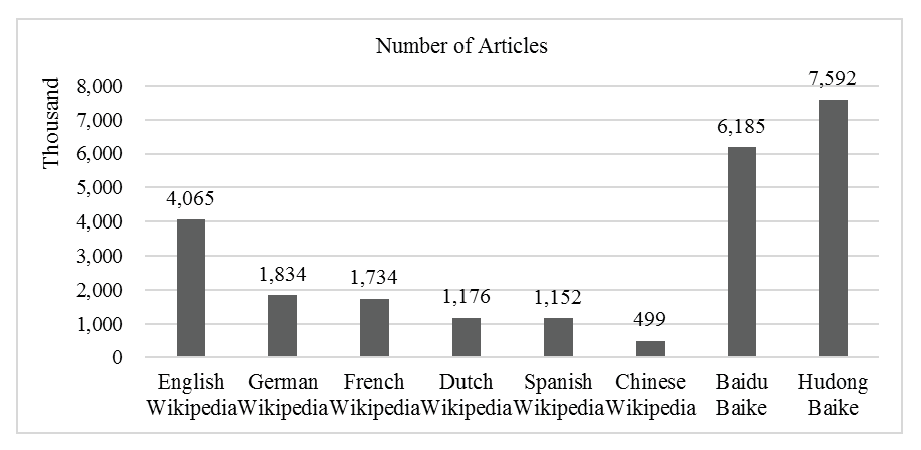
\includegraphics[width=0.8\columnwidth]{fig_stat}
  \caption{几个主要百科词条数量分布情况}
  \label{fig:wiki-stat}
\end{figure}

近年来,国内也涌现出一批通用领域的商业化百科全书,如百度百科\footnote{\url{http://baike.baidu.com/}}与互动百科\footnote{\url{http://www.baike.com/}}。这些在线百科经过数以万计的人员撰写修改,已经形成很大规模,积累了丰富的中文知识。其中互动百科作为目前中国最大的开放式网络百科全书,截止到2016年3月已收录词条超过1,430万条,远超过维基百科的中文词条数量。百度百科也有1313万个词条。如果能融合两个中文百科的信息,平衡中英文知识量级就可能实现。

%国内切实存在一些商业化的中文知识库,如搜狗“知立方”和百度“知心”,它们都是以人性化搜索、个性化推荐为出发点所建立的知识图谱产品。研究领域也有Zhishi.me\cite{niu2011zhishi} 等中文知识库。然而,随着开放链接的增多,人们发现单语言数据集已经不能满足语义万维网知识融合,知识共享的特点。除了更好的融合多语言知识,跨语言链接还用来辅助机器翻译\cite{niehues2011using}、跨语言信息检索\cite{giang2015building}等。然而因为维基中文知识匮乏,中英文难以对齐等原因,中英文的跨语言链接还很少。

\section{相关概念定义}
{\heiti 知识库}是大量知识的存储体,它将表征现实事物、分类、关系、规则、描述等的数据组织起来,成为计算机可理解的形式。知识库可以表示为$KB=<O,I>$,O为本体,I为实例集合,实例代表具体事物。

{\heiti 本体}则是对知识库概念体系的一种形式化说明,以概念、属性及其层次关系构成,定义为$O=<C,P,H^C,H^P>$,$C$为概念集合,概念是对相似实例抽象出的类别;$P$为属性集合,属性是对实例的描述,表征实例与其特征值的关系。$H^C$为概念上下位关系,$H^P$为属性层次关系,概念与属性共同构成了知识库的本体框架,对于描述事物起着重要作用。

%本体作为知识库的骨架,其准确性与完整性至关重要。通常,本体包含概念与属性,概念是对一些相似事物抽象出的类别,属性对事物特性进行描述。
%在RDF的定义中,有一些已定义的核心属性,如Rdf:type建立了实例与概念的instanceOf关系,也可以自定义属性。DBpedia有7000多个自定义属性,以\textit{http://nl.dbpedia.org/property}的形式定义。

维基百科的数据具有较为完备的结构化设计,其中的诸多元素与知识库元素相近,可以直接拿来辅助知识库本体的构建。比如其分类体系可以抽象成本体概念体系,其信息框属性可以作为自定义属性。

信息框是词条的“脸面”,包含了该词条的基本的代表性信息,读者通过阅读信息框,就可以了解关于词条的大部分重要内容。图\ref{fig:frozen-zhwiki-infobox-dump}左图中给出了中文维基词条\textit{冰雪奇缘}\footnote{https://zh.wikipedia.org/wiki/冰雪奇缘} 的信息框示例。信息框中通常以\textit{<属性-属性值>}的关系事实描述相应实体的特性,如果在知识库中将其作为实例的属性,则通过信息框增加的属性可达万级。

\begin{figure}[h]
  \centering
  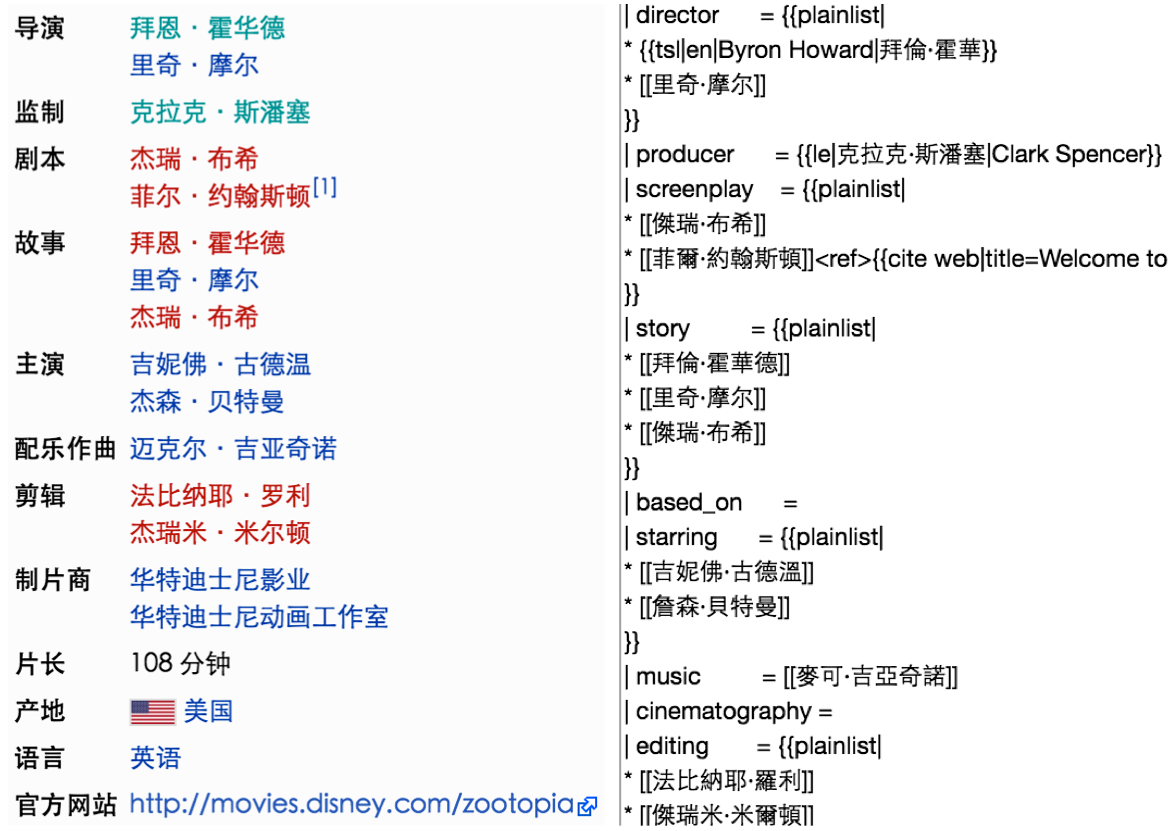
\includegraphics[width=0.6\columnwidth]{frozen-zhwiki-infobox-dump}
  \caption{动画电影\textit{冰雪奇缘}在中文维基中的信息框与编辑信息}
  \label{fig:frozen-zhwiki-infobox-dump}
\end{figure}

作为最常用的知识库数据源,维基百科词条中包含大量的信息框与属性信息。编辑者在撰写词条信息框时,以信息框模板(Infobox Template)作为指导,使用模板中提供的属性描述指定词条。图\ref{fig:frozen-zhwiki-infobox-dump}右图给出\textit{冰雪奇缘}的编辑源码,该词条信息框使用\textit{Infobox film}模板,为director,producer等属性赋值。知识库构建者可以充分利用这类结构化信息填充属性信息。此外,构成指定概念下的属性模板,将其进一步作为描述实例的指导,也是一件有意义之事。

\section{问题与挑战}

虽然目前跨语言知识图谱的构建已经有大量实践成果,并贡献了一定中英文对齐知识,但实现并完善一个高可用性的中英文知识库,依然存在很多问题,其中一项则为跨语言知识库本体的构建。

基于百科构建的知识库,通常会通过词条信息框补充属性。
哪些属性可描述同一概念下的一类实体?同一表达形式的属性是否表达着唯一含义?本体层概念与属性关系的定义与生成,对构建一个准确、可用的知识库起着重要作用。

而维基模板辅助一类词条的描述,融合了特定概念下的指定信息,对于生成概念属性有很好的借鉴作用。我们可以通过维基模板抽象出概念并合并相关属性形成概念模板。但维基经过多次更新换代,存有众多编辑者的修改痕迹,虽然发布了结构化信息,其数据却依然很复杂,尤其在信息框模板方面,具体表现在:
\begin{itemize}
\item {\heiti 模板标签与显示标签不一致}:由图\ref{fig:frozen-zhwiki-infobox-dump}右图可以看出,维基提供的的数据存储文件中,调用的模板中的属性标签(称之为模板标签)与真正显示在网页上的(称之为显示标签)不一致,这意味着仅仅解析存储文件并不能得到完整的属性信息,还需要更多辅助信息将两种标签对应上。
\item {\heiti 模板制定规则不统一}:维基百科为模板也单独成立一个词条页面,其中包含对模板属性集合的描述、使用方式等。我们发现维基对于信息框模板的定义不尽相同,从格式上来说,可分为键值对模板、表格模板等等。想要获得更全面的属性信息,需要区分不同类型的模板。
\end{itemize}

此外,在跨语言知识库构建过程中,本体对齐也是核心关注点。大部分跨语言知识库,如DBpedia、YAGO,都利用维基百科提供的跨语言词条链接来匹配多语言的实例与概念。维基百科没有直接提供属性跨语言信息,并且其发布的公开数据也不包含可用的信息框属性对齐关系。信息框属性链接的缺少,使得基于维基的跨语言本体在属性层无法匹配,知识库骨架无法形成。另外从知识量上说,中文维基属性信息与英文不对等,据最新统计,截止到2016年2月,维基带有信息框的英文词条数量约是中文词条的9倍,中文维基带有信息框的词条数量约为词条总量的1/4。如果仅仅依靠维基百科获得属性对齐关系,必然会受到维基中英文知识数量不平衡的极大限制。

如何获取更多的属性跨语言链接?引入其他数据源进行补充是可行方法之一。而异构百科带来了其他问题:
\begin{itemize}
\item {\heiti 异构百科编辑规则不一致},属性表示迥异,即使在同语言情况下,也有很多相同属性不能直接对齐。比如中文维基使用\textit{制片商},百度百科使用\textit{出品公司}作为电影制作公司属性的标签,中文维基常有\textit{旁白}、\textit{配乐作品}等百度百科不使用的属性。因此,仅依赖标签文本的对齐行不通,必须充分利用多源信息对知识进行查漏补缺、错误修正,面临的问题有所增多。
\item {\heiti 其他百科对于属性的概念界限划分模糊不清}。维基信息框模板很好地给定了描述一类实体的属性集合,而其他百科则不包含此类模板信息。面对无规则无限制的杂乱属性集,如何准确定义概念属性,制定特定领域下受认可的模板,从而更好地为属性对齐服务,是我们需要解决的难题。
\end{itemize}

属性分析,对实体准确描述、知识库本体构建起着重要作用。据我们所知,当前还没有中英文知识库对属性进行全面的分析与处理。如何定义概念与属性的关系,处理异构百科的跨语言属性对齐,完善中英文跨语言知识库,是当前亟需解决的问题。
本文对百科的信息框属性进行了概念定义、同义查找、跨语言对齐等研究,力求获得更准确的知识库本体,发现更多的跨语言链接。

\section{主要工作}
为解决中文知识匮乏问题,我们构建了大规模跨语言知识图谱XLore\footnote{\url{http://xlore.org}},充分利用异构中、英文在线百科丰富的信息,将中英文维基、百度百科、互动百科中的词条、分类与信息框分别抽象成知识库中的实例、概念和属性,并利用维基的语言链接信息与链接扩展方法\cite{wang2012cross},添加双语知识关系,成功将双语语义信息融合在一起,为中英文知识共享打下了基础。

然而,XLore中虽然含有来自四个百科数据源的约6万个属性,但并没有进行很好的区分,以及进一步的跨语言对齐处理。本文以完善跨语言知识图谱,构建规范本体为目标,着重对本体的概念与属性进行研究,尝试解决概念属性生成、跨语言对齐等问题,提高中英文信息的融合度。此外,从知识库应用角度出发,搭建展示系统与实体链接接口。本节根据之前提出的挑战,对涉及到的研究点进行了概括。

\subsection{维基百科概念属性生成}
对于基于维基百科生成的知识库,针对其概念以及概念属性集合问题,我们利用维基百科中现有的信息框模板抽象概念,并生成概念属性。通过分析信息框模板,我们获取了维基百科大部分概念属性,可覆盖维基中90\%以上的词条的信息框,为后续对概念属性的进一步研究打下了良好基础。

\subsection{异构百科跨语言属性对齐}
不同于大多数的跨语言属性对齐研究,本文中以领域信息区分不同概念下相同标签的属性,同时进行百科异构性的分析,即对属性的研究建立在维基百科与百度百科两个百科上。结构与语言的双重障碍,为属性对齐的研究增加了难度。为尽可能达到结构上的统一,我们对无模板的百度百科属性集合进行领域划分,形成概念模板,并将属性对齐问题限定在概念领域范围下,同时利用中文维基为英文维基与百度百科搭桥引线,获取更多关联信息。总结来讲,本问题通过四个步骤解决并优化,分别为:1)生成百科概念属性模板,2)同语言对齐与相似属性合并,3)跨语言种子集合生成,4)跨语言属性对齐。

\subsection{中英文跨语言知识库系统与应用}
本文提及的知识库系统XLore,其构建初衷是为解决中文知识匮乏问题,提高知识融合度与共享率。为此我们将目光聚焦在国内信息最丰富的两大中文在线百科——百度百科与互动百科上,利用两大百科的词条页面信息、分类体系数据,并结合维基百科对外发布的数据存储文件,抽取语义信息,构成跨语言知识库XLore。值得一提的是,我们对XLore知识库的应用层面上也进行了尝试,主要体现在支持数据访问的在线系统XLore.org,以及提供实体语义信息的API接口,该接口支持限定领域查询与通用领域实体查询。

\subsection{主要贡献}
本文提出了一种概念属性生成与领域跨语言属性对齐的方法,应用在通用领域的中英文知识库XLore上,其中主要贡献列举如下:
\begin{enumerate}[1)]
\item {\heiti 维基百科概念属性生成,} 总结维基百科信息框模板与属性特点,制定相应抽取方法,从中生成概念属性集合,该集合覆盖了90\%以上的百科词条描述信息。
\item {\heiti 异构百科下的跨语言概念属性对齐,} 对英文维基百科与百度百科两个异构百科下的概念属性做对齐。包括百度百科下概念模板生成,同语言属性对齐,限定概念下的跨语言属性匹配。
\item {\heiti 为跨语言知识库XLore提供多元化的数据展示与应用接口,}前者分别从一般用户与专业用户的不同角度,给出搜索框查询与SPARQL查询两种知识访问方式;后者考虑知识库的应用场景,提供基于RESTFul的实体访问API,对给定文本进行实体分析与排歧,返回实体语义信息,该接口成功地应用于学术搜索和新闻挖掘领域。
\end{enumerate}

\section{论文组织}

本章对本文研究背景进行描述,总结了需要解决的挑战性问题,并概要地介绍了研究内容和主要贡献。如图\ref{fig:organization}所示,接下来的章节关系与结构组织如下:

\begin{figure}[ht] 
  \centering
  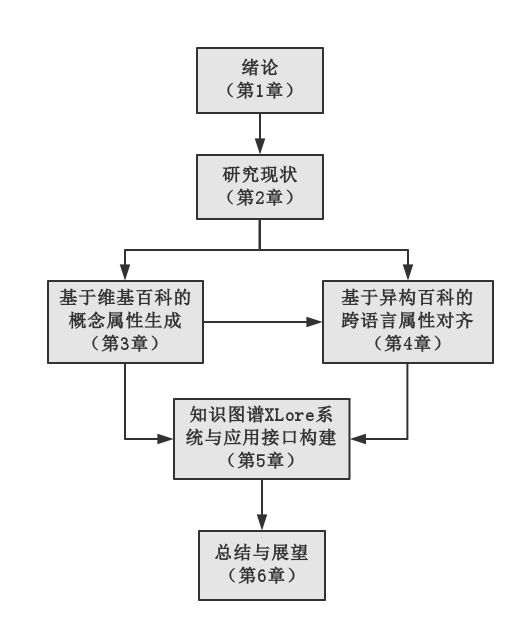
\includegraphics[width=0.65\columnwidth]{organization}
  \caption{论文组织结构图}
  \label{fig:organization}
\end{figure}

第 2 章为研究现状,介绍当前构建的跨语言知识图谱的发展情况,列举现今广为人知的多语言与中文单语言知识图谱,并介绍其构建技术;对跨语言本体对齐研究现状进行描述,包括本体对齐,属性对齐等。

第 3 章详细分析了维基百科的信息框制定规则,对数据文件中的模板给出了分类与处理方法,以覆盖大部分词条描述为目标,借由模板生成概念属性。

第 4 章说明了基于异构百科的跨语言属性对齐流程。首先通过观察与抽取百科中的模板与属性,提出异构百科属性研究的种种难点,之后为百科属性集合提取概念属性模板,并实现在特定领域下,同语言相似属性的对齐与跨语言属性链接。

第 5 章简要介绍了基于多源异构在线百科构建跨语言知识图谱XLore的过程,重点展示了系统可视化与数据访问接口,并从实际应用角度展示其可用性。

第 6 章对本文提出的跨语言属性对齐与知识图谱构建和应用研究工作进行了总结和展望,分析了不足之处,为进一步研究提出了新的方向。

